\chapter{Project Management}
\label{Project_Management}

\section{Deliverables and milestones}

Our experience from fall and winter quarter supports our notion that a detailed forward-thinking plan is necessary for creating high quality work. Taking this experience into account we decided to meet together at the beginning of each week during spring quarter explicitly to plan our actions for that week. In order to deduce what had to be done each week we filled out a calendar backwards starting at the date of EXPE and heading back to the beginning of spring quarter. Allowing for ample spill over time should any one goal have unexpected challenges, we assigned deadlines which, if followed, would ensure that we would have a well finished prototype for EXPE.\\
At each weekly meeting, we would recap what we finished in the previous week to ensure everyone in the group was aware of what everyone else was doing and what needed to get done in the following week. Though not a perfect system, we found that these weekly planning meetings were the best method for ensuring that our team stayed on track for EXPE.\\
Below is a recap of the main milestones and deliverables that led us towards our final prototype that we presented on EXPE. 

\begin{figure}[h]
  \centering
     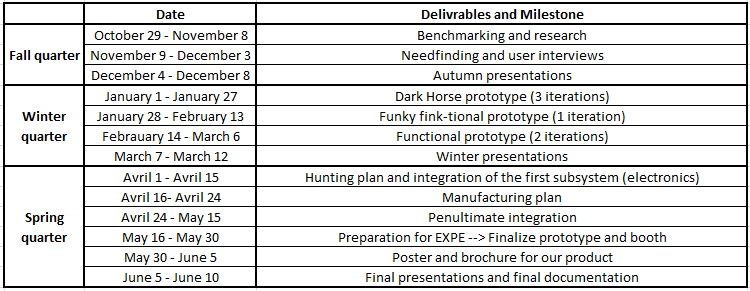
\includegraphics[scale=0.8]{images/planning.png}
   \caption{Deliverables and Milestones for the whole project}
  \label{fig:planning}
\end{figure}


\section{Distributed team management}

Over the past three quarters the seven of us have learned a lot of lessons about how to work together as a distributed team and how to take advantage of our diverse talents. Our diverse backgrounds (two mechanical engineers, one aerospace engineer, one product designer, two industrial engineers and one electrical engineer) allow each of us to shine in various ways. During winter and spring quarter we have challenged each other to take on something outside of their individual comfort zones, with some successes and some failures…\\

In order to ensure a successful cooperation inside the team, we decided to set a weekly meeting for the winter and spring quarter with our global partner. We thought it was a very useful update on what each entity of the team had worked on during the week. It was also a valuable safety net when the schedule started to get very busy. In addition to these regular meetings, we also shared our documentation and our work on a Podio platform. It enabled us to share content and react almost immediately to our peers’ ideas. When discussions were required between individuals who were collaborating, we used Skype as an informal and easy way to share ideas.\\

We believed that another attribute of our success as a team is the relationship that we built during the Stanford’s team visit to USP in March. The social connection and a good understanding allowed us to feel comfortable both to tease each other and to throw out crazy ideas which challenged the group.


\section{Project Budget}

\subsection{Stanford Budget}

\subsection{USP Budget}
 
\section{Reflection and Goals}

\subsection{Stanford Team}

\subsubsection{Clifford Bargar}

\subsubsection{Maria Barrera}

\subsubsection{Laura Hoinville}

This project was a great experience. I must admit it took me some time to understand what the expectations both from the class and from our users were. ME 310 was my first product design class and it made me realize how important it is to understand who your user is and how to put yourself in their shoes to make sure you your solution addresses their real problems. This project was a great opportunity to merge my engineering skills (I’m from an aerospace engineering background) with empathy and understanding of the needs and issues of people we were designing for.\\

I know a lot of aircraft design because this is the field where I’d like to start my career, but anytime I was taught about it, it was mainly in terms of aircraft performance and never in terms of people’s need. I think this project enabled me to see aircraft design from the user’s point of view instead of the aircraft manufacturer’s point of view and for me this was extremely valuable.//
Since I come from France it was actually the first time that I had the opportunity to work with both American and Brazilian people and this cultural diversity was also a great source of enrichment.\\

But beyond this, this project now means a lot to me. I got the opportunity to talk to disabled people and understand how painful it is for them to travel. They care a lot about our project because they see it as a way to improve their experience and I did not want to disappoint them. They deserve the right to enjoy their flights the way we do and for this reason I’m very excited to see what Embraer will do with our prototype and our work and I hope this will contribute in making the flying experience more enjoyable for people with reduced mobility. 


\subsection{USP Team}

\subsubsection{Luiz Durao}

\subsubsection{Guilherme Kok}

\subsubsection{Rodrigo Monteiro}

\subsubsection{Amanda Mota}

